\chapter[Referencial Teórico]{Referencial Teórico}
\label{ch:referencial_teorico}

Nesta seção serão apresentados os principais conceitos utilizados neste trabalho, sendo eles: motores de corrente contínua; Filtro de \emph{Kalman}; Método dos mínimos quadrados; Introduz alguns conceitos chaves sobre a teoria de controle; Breve explicação sobre a comunicação \emph{Bluetooth}; Detalhes sobre o funcionamento dos \emph{Encoders} rotativos incrementais e por fim fala sobre o funcionamento básico dos sinais PWM.
%********************************************************************
\section{Motor de Corrente Contínua}
\label{sec:motor_ref_teo}
% Introduzir o que funcionamento básico de um motor CC
% deixar claro qual o tipo será apresentado/utilizado no trabalho (motor CC de campo magnético fixo e com "escova")
Como o próprio nome indica, os motores CC são acionados por uma fonte de corrente contínua. Esse tipo de motor é amplamente utilizado em diversas aplicações.

Ele é constituído basicamente pelo enrolamento de armadura, enrolamento de campo ou ímãs permanentes, comutador e as escovas, onde:

\begin{itemize}
    \item Enrolamento de armadura: é localizado na parte giratória do motor de CC (rotor) que é responsável por produzir o torque que o movimenta, bem como a tensão de saída quando em modo de gerador.
    
    \item Enrolamento de campo: parte fixa responsável pelo fluxo magnético constante que irá atravessar a armadura. Em motores CC de pequenas dimensões, como os utilizados neste trabalho, o enrolamento de campo muitas vezes é substituído pela colocação de ímãs permanentes ao redor da armadura, responsáveis por gerar um campo magnético constante.
    
    \item Comutador: Possui a função de manter a corrente da armadura circulando no mesmo sentido, fazendo com que o torque mantenha seu sentido para uma tensão de entrada constante.
    
    \item Escovas: é por onde acontece o contato do enrolamento de armadura com a fonte de alimentação.
\end{itemize}


As máquinas de corrente contínua são bastante utilizadas em sistemas de controle em razão do seu comportamento essencialmente linear. O diagrama esquemático de uma máquina (motor ou gerador) CC é mostrado na figura \ref{fig:modelo_motor_dc}. O enrolamento de campo tem resistência $R_f$ e indutância $L_f$ e o enrolamento de armadura tem resistência $R_a$ e indutância $L_a$. As correntes e tensões nos enrolamentos de campo e de armadura $i_f$, $v_f$, $i_a$ e $v_a$, respectivamente. A tensão induzida na armadura é $v_g$. O torque e a velocidade angular no eixo do rotor são $\tau$ e $\omega$, respectivamente.

A tensão induzida no enrolamento de armadura é dada por:

\begin{equation}
    v_g = K_{1}\phi\omega
\end{equation}

E o torque é dado por:

\begin{equation}
    \tau = K_{1} \phi i_a 
\end{equation}onde $K_1$ é um parâmetro determinado pela estrutura física da máquina e $\phi$ é o fluxo magnético. Supondo que a máquina esteja operando na zona linear (ou seja, que o núcleo não esteja saturado), o fluxo é dado pela equação:
\begin{equation}
    \phi = K_{2}i_f
\end{equation}onde $K_2$ é uma constante e depende das características magnéticas do núcleo e do enrolamento de campo. No caso de motores com ímãs permanentes, o fluxo $\phi = \phi_\text{const}$ é constante, determinado pelos materiais e características de construção dos ímãs.

Motores geram potência mecânica, de forma que a velocidade de rotação $\omega$ é o sinal de saída e a tensão $v_a$ aplicada é o sinal de entrada. 

\begin{figure}[H]
    \centering
    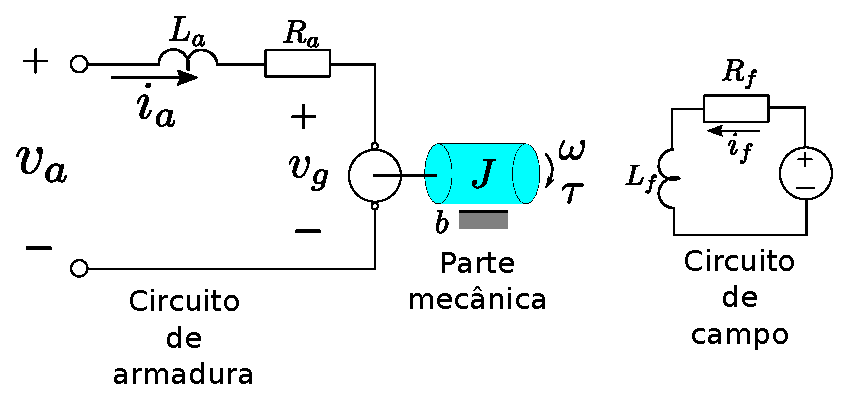
\includegraphics[width=0.5\textwidth]{figuras/ilustracoes/esquematico_motor_dc.eps}
    \caption{Diagrama esquemático de um motor CC.}
    \label{fig:modelo_motor_dc}
    \fonte{Própria.}
\end{figure}


A Figura \ref{fig:modelo_motor_dc} apresenta o diagrama esquemático para um motor de corrente contínua (CC) controlado pela armadura, ou seja, o sinal de entrada é a tensão aplicada na armadura ($v_a$). Nesse diagrama a carga está sendo modelada por um momento de inércia $J$ e um atrito viscoso de coeficiente $b$.

\begin{align*}
    v_g &= K_{1}\phi\omega= K_{1}K_{2}i_{f}\omega = K_{m}\omega\\
    \tau &= K_{1} \phi i_{a}= K_{1} K_{2}i_{f} i_{a} = K_{m}i_{a}
\end{align*}

A constante $K_{m}$ é conhecida como a constante do motor. Devido à relação apresentada anteriormente é possível modelar o circuito equivalente do motor CC como na imagem \ref{fig:eq_eletrico_motorcc}.
% figura baseada na fig. do livro texto da disciplina de modelagem.
\begin{figure}[H]
    \centering
    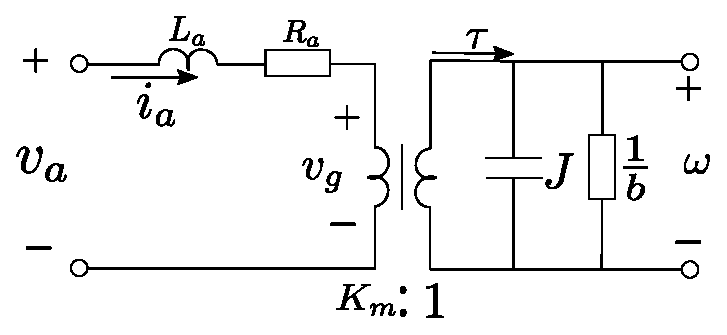
\includegraphics[width=0.6\textwidth]{figuras/ilustracoes/circuito_equivalente_motor_cc.eps}
    \caption{Equivalente elétrico de um motor CC}
    \label{fig:eq_eletrico_motorcc}
    \fonte{Própria.}
\end{figure}

Do circuito da figura \ref{fig:eq_eletrico_motorcc} extrai-se a seguinte função de transferência:

\begin{equation*}
    \frac{\Omega(s)}{V_a(s)} = \frac{K_m}{JL_{a}s^2 + \left(JR_a + BL_a \right)s + BR_a + K_{m}^2} \left[\frac{ rad.s^{-1}}{V}  \right]
\end{equation*}

Caso a impedância da armadura seja desprezada $(L_a \xrightarrow{} 0)$, o que quase sempre é possível pois a constante de tempo relacionada ao comportamento mecânico do motor é muito maior do que a relacionada ao funcionamento elétrico:

\begin{equation}
    \frac{\Omega(s)}{V_{a}(s)} = \frac{K_m}{JR_{a}s + BR_{a} + K_{m}^2} = \frac{K}{T_{m}s + 1} \left[\frac{ rad.s^{-1}}{V}  \right]
    \label{eq:motor_transf_func}
\end{equation}

Portando, caso a impedância da armadura seja desprezada, a função de transferência do motor que relaciona a velocidade angular com a tensão de entrada se comporta como a de um sistema de primeira ordem. A maior dificuldade encontrada ao se controlar motores CC é a amplitude elevada da corrente de armadura, o que requer a utilização de sinal $v_a$ de entrada fornecido por uma fonte de alta potência.
\input{textuais/referenciais_teoricos/sistemas_de_primeira_ordem}
\section{Sistemas de Controle}
\label{sec:sistema_controle}
O controle automático é um componente importante e intrínseco em sistemas de veículos espaciais, sistemas robóticos, modernos sistemas de manufatura e quaisquer operações industriais que envolvam o controle de temperatura, pressão, umidade, viscosidade, vazão etc \cite{ogata2011engenharia}. Um problema de controle consiste em determinar uma forma de afetar um dado sistema físico de modo que seu comportamento atenda às especificações de desempenho previamente estabelecidas. Como, normalmente, não é possível alterar a estrutura funcional do sistema físico em questão, a satisfação das especificações de desempenho é atingida mediante o projeto e implementação de controladores.


\textbf{Sistema de controle em malha aberta (\emph{Feedforward}).} Sistema de controle que não possui a entrada influenciada pela saída do sistema. Isso quer dizer que o sinal de saída não é medido nem realimentado para comparação com a entrada (Ver Figura \ref{fig:ilustracao_sistema_malha_aberta}). Devido à natureza desse tipo de controle, a entrada de referência é mapeada para uma saída correspondente do controlador. Dessa maneira, a precisão do sistema depende de uma calibração para melhor ajustar/mapear a referência em um determinado sinal de controle.

\begin{figure}[H]
    \centering
    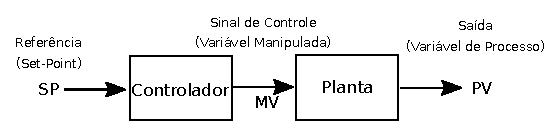
\includegraphics[width=0.8\textwidth]{figuras/ilustracoes/diagrama_sistema_malha_aberta.eps}
    \caption{Diagrama de exemplificação de sistema de controle em malha aberta.}
    \label{fig:ilustracao_sistema_malha_aberta}
    \fonte{Própria.}
\end{figure}

\textbf{Sistema de controle em malha fechada.} Difere essencialmente do em malha aberta, pois neste tipo a entrada do controlador é influenciada pela saída do sistema de controle (variável de processo), (Ver Figura \ref{fig:ilustracao_sistema_malha_fechada}). Esse tipo de sistema de controle também é denominado de controle com realimentação. A relação entre a saída e a entrada de referência se dá por meio da comparação entre elas, utilizando a diferença como meio de controle.

\begin{figure}[H]
    \centering
    \includegraphics[width=0.8\textwidth]{figuras/ilustracoes/diagrama_sistema_malha_fechada.eps}
    \caption{Diagrama de exemplificação de sistema de controle em malha fechada.}
    \label{fig:ilustracao_sistema_malha_fechada}
    \fonte{Própria.}
\end{figure}


Segundo \cite{ogata2011engenharia} as principais vantagens do sistema de controle em malha aberta são:
\begin{enumerate}
    \item São de fácil construção/implementação e fácil manutenção.
    \item Não apresentam problemas de estabilidade.
    \item São mais adequados em situações em que a medição precisa da saída é um problema.
\end{enumerate}

E algumas desvantagens:

\begin{enumerate}
    \item Distúrbios e mudanças na calibração causam erros, e a saída pode apresentar diferenças
    em relação ao padrão desejado.
    \item Para que a saída mantenha a qualidade requerida, é necessária uma regulagem periódica.
\end{enumerate}


\subsection{Controlador PID}
% Controlador PID
% Controlador malha aberta Feedforward
Um controlador clássico do tipo \emph{Feedback} e que ainda é muito utilizado é o controlador proporcional Integral derivativo (PID). Como o próprio nome indica, esse tipo de controlador une as ações derivativa, integral e proporcional. De maneira simplificada, a ação proporcional faz com que o erro diminua e influencia no tempo de resposta do sistema, a ação integral elimina o erro de regime e a ação derivativa influencia no tempo de resposta do sistema, por meio da antecipação do erro.

Definindo-se os seguintes sinais no tempo: $u(t)$ como sinal de saída (sinal de controle) e $e(t)$ como o erro entre a referência e o valor atual da saída da planta, o controlador pode ser definido como:

\begin{equation}
    u(t) = K_{p}e(t) + K_{i} \int^{t}_{0}e(\tau)d\tau + K_{d}\frac{d e(t)}{dt}
\end{equation}

Aplicando a transformada \emph{Laplace} temos,

\begin{equation}
    \frac{U(s)}{E(s)} = K_{p} + \frac{K_{i}}{s} + K_{d}s
\end{equation}

Sendo,

\begin{itemize}
    \item $K_p$: O ganho proporcional.
    \item $K_i$: Ganho integral.
    \item $K_d$: Ganho derivativo.
    \item $s$: Frequência complexa.
\end{itemize}

Esse tipo de controlador pode ser utilizado em mais três formas básicas além do padrão PID: Controle Proporcional (P). Apenas a ação proporcional; Controle Proporcional Integral (PI) e Controle Proporcional Derivativo (PD).

\begin{figure}[H]
    \centering
    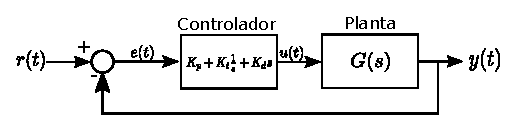
\includegraphics[width=\textwidth]{figuras/ilustracoes/diagrama_controlador_PID.eps}
    \caption{Diagrama de um sistema controlado por PID.}
    \label{fig:diagrama_controlador_PID}
    \fonte{Própria.}
\end{figure}

A Figura \ref{fig:diagrama_controlador_PID} ilustra em diagrama de blocos o uso do controlador PID. Onde $r(t)$ é o sinal de referência (\emph{set-point}), $y(t)$ é a saída da planta e $G(s) = Y(s)/U(s)$ é a função de transferência da planta.

\subsection{Sistemas de Primeira Ordem}

Um sistema de primeira ordem apresenta a seguinte forma genérica:

\begin{equation}
    T\dot{y} + y = Ku
\end{equation}

e em \emph{Laplace} com a seguinte função de transferência,

\begin{equation}
    G(s) = \frac{K}{Ts + 1}
\end{equation}

e sua resposta no tempo para uma entrada do tipo degrau unitário,

\begin{equation}
    y(t) = K \left(1 - e^{-t/T} \right)
\end{equation}

Sendo $K$ o ganho do sistema e a constante $T$ é conhecida como constante de tempo do sistema e $T > 0$. A Figura \ref{fig:saida_sistema_primeira_ordem_no_tempo} ilustra o comportamento no tempo de um sistema de primeira ordem e a influência da constante de tempo $T$ na resposta do sistema.

\begin{figure}[H]
    \centering
    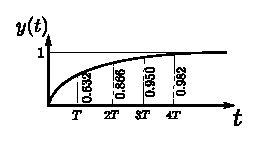
\includegraphics[width=0.5\textwidth]{figuras/ilustracoes/resposta_no_tempo_sistema_primeira_ordem.eps}
    \caption{Resposta no tempo ao degrau unitário de um sistema de primeira ordem com ganho unitário e contante de tempo $T$.}
    \label{fig:saida_sistema_primeira_ordem_no_tempo}
    \fonte{Própria.}
\end{figure}

% O erro de regime é a diferença entre os sinais de entrada e de saída na região de regime da resposta. Ou seja, $t \xrightarrow{} \infty$.
\section{Mínimos Quadrados}
\label{sec:MMQ}

O Método dos Mínimos Quadrados (MMQ) é uma técnica de otimização matemática que procura encontrar o melhor ajuste para um conjunto de dados por meio da minimização da soma dos quadrados das diferenças entre os valores estimados e os observados (tais diferenças são chamadas resíduos).

Um requisito para o método dos mínimos quadrados é que o erro possua uma distribuição normal. Outro requisito é que as variáveis devem apresentar uma relação linear entre si \cite{MMQ}.

Ao usar uma base de dados com $k$ variáveis explicativas ($x$) e $n$ observações ($y$), o modelo pode ser escrito na forma matricial:

% A regressão múltipla leva em consideração diversas variáveis explicativas $x$ influenciando $y$ ao mesmo tempo \cite{wiki:MMQ} e o formato do 

\begin{equation}
    \bm{Y} = \bm{X\alpha{} + e}
\end{equation}
onde as matrizes possuem a seguinte forma:

\begin{align*}
    \bm{Y} =
    \begin{bmatrix}
        y_1\\
        y_2\\
        \vdots\\
        y_n
    \end{bmatrix},
    \bm{X} = 
    \begin{bmatrix}
        1 & x_{11} & x_{21} & \hdots & x_{k1} \\
        1 & x_{12} & x_{22} & \hdots & x_{k1} \\
        \vdots & \vdots & \vdots & \vdots & \vdots \\
        1 & x_{1n} & x_{2n} & \hdots & x_{kn}
    \end{bmatrix} \times 
    \begin{bmatrix}
        b_0\\
        b_1\\
        \vdots\\
        b_k
    \end{bmatrix},
    \bm{e} = 
    \begin{bmatrix}
        e_1\\
        e_2\\
        e_3\\
        \vdots\\
        e_n
    \end{bmatrix}
\end{align*}
, onde $x_{ji}$ representa o valor da $j$-ésima variável da $i$-ésima observação.

A solução de mínimos quadrados se dá através da minimização da soma do quadrado dos resíduos conforme apresentado em \cite{wiki:MMQ} e o resultado é apresentado na Equação \ref{eq:MMQ_solucao}.

\begin{equation}
    \bm{\hat{\alpha}} = \bm{\left( X^{T}X \right)^{-1}X^{T}Y}
    \label{eq:MMQ_solucao}
\end{equation}
sendo $\bm{\hat{\alpha}}$ a melhor estimativa para os parâmetros que relacionam $\bm{X}$ com $\bm{Y}$.

Por exemplo, para se realizar uma regressão de um conjunto de observações com o seguinte comportamento linear:

\begin{equation}
    y = b + ax
\end{equation}
podemos arranjar os dados na forma matricial:

\begin{equation*}
    \bm{Y} = \bm{X\alpha}
\end{equation*}
sendo,

\begin{align*}
    \bm{Y} =
    \begin{bmatrix}
        y_1\\
        y_2\\
        \vdots\\
        y_n
    \end{bmatrix},
    \bm{X} = 
    \begin{bmatrix}
        1 & x_1\\
        1 & x_2\\
        \vdots & \vdots\\
        1 & x_n
    \end{bmatrix}, 
    \bm{\alpha} = 
    \begin{bmatrix}
        b\\
        a
    \end{bmatrix}
\end{align*}
com isso podemos calcular a melhor estimativa $\bm{\hat{\alpha}} = \begin{bmatrix}\hat{b} & \hat{a}\end{bmatrix}^T$ como em \ref{eq:MMQ_solucao}.

\begin{comment}
De maneira geral, a ideia por trás do método dos mínimos quadrados (MMQ) é de encontrar os coeficientes da(s) função(ões) de base que minimizem o erro, ou seja, com o menor erro possível associado à representação \cite{MMQ}. Assim, dado que queremos obter a equação e possuímos vetores de dados $x$ e $y$, e queremos relacioná-los. Por exemplo, caso queira-se aproximar o conjunto de dados para a reta:

\begin{equation}
    y = ax + b.
    \label{eq:pol1}
\end{equation}

Teremos a seguinte relação para o MMQ.

\begin{align*}
    \textbf{Y} = \textbf{X}\alpha
\end{align*}
% \[\textbf{Y} = \textbf{X}\alpha\]
sendo,

\begin{equation*}
    \textbf{Y} =
    \begin{bmatrix}
     y_1\\
     y_2\\
     \vdots\\
     y_n
    \end{bmatrix},
    \textbf{X} = 
    \begin{bmatrix}
        x_1 & 1\\
        x_2 & 1\\
        \vdots & \vdots\\
        x_n & 1\\
    \end{bmatrix},
    \bm{\alpha} =
    \begin{bmatrix}
        a\\
        b\\
    \end{bmatrix}
\end{equation*}

A ideia por trás do método de mínimos quadrados é minimizar o erro $\bm{e}$. Sabendo que o espaço gerado por tal plano ortogonal será dado pela matriz $\bm{X^T}$, então queremos impor que o vetor de erro $\bm{e}$ será nulo, logo:

% \[\textbf{X}^T\textbf{e} = \textbf{0}\]

\[\bm{X^T e = 0}\]

Como,

% \[\textbf{e} = \textbf{Y} - \textbf{X}\hat{\alpha}\]
\[\bm{e = Y - X\hat{\alpha}}\]

Então temos,

\[\textbf{X}^T(\textbf{Y} - \textbf{X}\hat{\alpha})= \textbf{0}\]
\[\bm{\hat{\alpha}} = (\textbf{X}^T\textbf{X})^{-1}\textbf{X}^T\textbf{Y} \]

Sendo,

\[\bm{\hat{\alpha}} =
\begin{bmatrix}
 \hat{a}\\
 \hat{b}\\
\end{bmatrix}
\]

Os elementos do vetor $\bm{\hat{{\alpha}}}$ serão os coeficientes da equação \ref{eq:pol1} que minimizarão o erro, ou seja, são os coeficientes da reta que melhor representam o conjunto de dados.
\end{comment}
\section{Filtro de Kalman}
% Introdução ao filtro de Kalman
\label{sec:kalman}
"A filtragem de \emph{Kalman} é um processo de estimativa de estado ótimo aplicado a um sistema dinâmico que envolve perturbações aleatórias. Mais precisamente, o filtro de \emph{Kalman} fornece um  procedimento recursivo linear, imparcial e que visa minimizar a variância do erro para estimar de forma otimizada o estado desconhecido de um sistema dinâmico de dados ruidosos obtidos em tempo real discreto. Tem sido amplamente utilizado em muitas áreas de aplicações industriais e governamentais, como sistemas de rastreamento, navegação por satélite, estimar trajetória de mísseis balísticos e radar." \cite{kalman:book}.\\

O filtro de \emph{Kalman} usa um modelo dinâmico do sistema (por exemplo, leis físicas do movimento), entradas de controle conhecidas para esse sistema e várias medições sequenciais (como de sensores) para formar uma estimativa das quantidades variáveis do sistema (seu estado $\textbf{x}_k$) que é melhor do que a estimativa obtida usando apenas as medições. Como tal, é um algoritmo comum de fusão de sensores e fusão de dados \cite{kalman:wiki}, \cite{Kalman:ofid}.\\

O filtro produz uma estimativa do estado do sistema como uma média do estado previsto do sistema e da nova medição usando uma média ponderada. O objetivo dos pesos é que os valores com menor incerteza sejam mais "confiáveis". O ganho de \emph{Kalman} é o peso relativo dado às medições e estimativa do estado atual.\\

Para o uso do filtro de \emph{Kalman} deve-se modelar o processo de acordo com a seguinte estrutura. Isso significa especificar as seguintes matrizes \cite{kalman:book}:

\begin{itemize}
    \item $\textbf{F}_k$: Modelo de transição de estado.
    \item $\textbf{H}_k$: Modelo de Observação.
    \item $\textbf{Q}_k$: Covariância do ruído do processo.
    \item $\textbf{R}_k$: Covariância do ruído da observação(medição).
    \item $\textbf{B}_k$: Modelo de entrada de controle (caso o sistema dinâmico tenha entrada). 
\end{itemize}


Modelo do sistema para o filtro de \emph{Kalman}:
\begin{equation}
\textbf{x}_k = \textbf{F}_x \textbf{x}_{k-1} + \textbf{B}_k \textbf{u}_k + \textbf{w}_k; \textbf{w}_k \sim N(0, \textbf{Q}_k)
\end{equation}

Sendo $\textbf{w}_k$ o ruído de processo, que assume-se ter uma distribuição normal de média zero e covariância $\textbf{Q}_k$. ($\textbf{w}_k \sim N(\textbf{0}, \textbf{Q}_k)$).

Modelo da observação/medição será:
\begin{equation}
\textbf{z}_k = \textbf{H}_k \textbf{x}_k + \textbf{v}_k; \textbf{v}_k \sim N(\textbf{0}, \textbf{R}_k)
\end{equation}

Sendo $\textbf{v}_k$ o ruído de observação, que assume-se ser um ruído gaussiano branco de média zero e covariância $\textbf{R}_k$. ($\textbf{v}_k \sim N(\textbf{0}, \textbf{R}_k)$).

A filtragem é frequentemente dividida como duas fases: Predição e Atualizar (Alguns autores também contam a etapa de medição como uma fase do algoritmo). A fase de predição usa a estimativa anterior para produzir uma estimativa do estado atual. Na fase seguinte (de atualização), a predição atual é combinada com as informações da medição atual para aprimorar a estimativa do estado. As etapas do filtro são apresentadas a seguir.

\textbf{Predição}:
\begin{align*}
    \check{\textbf{x}}_k &= \textbf{F}_k \hat{\textbf{x}}_{k-1} + \textbf{B}_k \textbf{u}_k\\
    \check{\textbf{P}}_k &= \textbf{F}_k \hat{\textbf{P}}_{k-1} \textbf{F}^T_k + \textbf{Q}_k
\end{align*}

Sendo $\check{\textbf{P}}$ uma predição da covariância do estado seguinte (predito, $\textbf{x}_k$).

\textbf{Atualização}:
\begin{align*}
    \textbf{K}_k &= \check{\textbf{P}}_k \textbf{H}^T \left( \textbf{H}_k \check{\textbf{P}}_k \textbf{H}^T_k + \textbf{R}_k\right)^{-1}\\
    \hat{\textbf{x}}_k &= \check{\textbf{x}}_k + \textbf{K}_k\left( \textbf{z}_k - \textbf{H}_k \check{\textbf{x}}_k \right)\\
    \hat{\textbf{P}}_k &= \left(\textbf{I} - \textbf{KH}_k \right)\check{\textbf{P}}_k
\end{align*}

Uma observação importante sobre a etapa de atualização é que ela irá tender para o valor predito caso o ganho do filtro $\textbf{K}_k$ seja baixo (resultado de um alto erro na medição). O contrário também ocorre, ou seja, para medições precisas ($\textbf{R}_k$ baixo) o ganho do filtro tende a ser alto e a etapa de atualização vai tender a usar mais a informação da medição como estado ótimo ($\hat{\textbf{x}}$). 

\section{\textit{encoders} Incrementais}
\label{sec:encoders}
% Referencias:
% https://www.roboticsbusinessreview.com/news/differences-between-encoder-resolution-accuracy-and-precision/
% https://www.newtoncbraga.com.br/index.php/como-funciona/5454-mec128
% [Speed Measumment Using Rotary encoders for High Performance ac Drives]
% [Speed Measurement Algorithms for Low-Resolution Incremental encoder Equipped Drives: a Comparative Analysis]
% [A Simple Speed Feedback System for Low Speed DC Motor Control in Robotic Applications]
% [An Embedded System for Position and Speed Measurement Adopting Incremental encoders]

% FALAR SOBRE O FUNCIONAMENTO BASICO
% CITAR OS DIFERENTES TIPOS
% FALAR DO GRAY CODE
% FALAR DO ERRO DE QUANTIZAÇÃO

As saídas de um \emph{encoder} incremental são, normalmente, duas ondas quadradas defasadas em $90^\circ$ uma da outra (em quadratura). Essa diferença de fase nos permite medir o sentido de rotação. Abordagens mais eficientes de leitura desses sensores são por meio da detecção das bordas dessas ondas, pois isso permite quadruplicar o número de pulsos por revolução (NPR) \cite{quantization_error01}. Existem dois métodos básicos para se realizar a medição da velocidade por meio desses sensores, são eles: \textbf{frequencímetro} e \textbf{periodímetro}. 

Na medição por frequência (\textbf{frequencímetro}), conta-se o número de pulsos que ocorreram em um determinado período de tempo fixo. Com isso a velocidade pode ser obtida pela seguinte aproximação:

\begin{equation}
    \omega = \frac{d\theta}{dt} \cong \frac{\Delta{\theta}}{T} \cong \frac{2 \pi \Delta{N}}{N_{PR}T}[rad.s^{-1}] \xrightarrow{} \frac{60 \Delta{N}}{N_{PR} T} [RPM]
\end{equation}

Sendo $N_{PR}$ o número de pulsos por revolução e $\Delta{N}$ é o número de pulsos que aconteceram dentro da janela de tempo $T$. Existe um erro de quantização nesse método de leitura devido à variação de ângulo medida ser sempre um múltiplo inteiro de $ 2\pi/N_{PR}$. O erro de quantização $\Delta{\omega}$ pode ser modelado pela seguinte equação:

\begin{equation}
    \Delta{\omega} = \frac{2\pi}{N_{PR}T}[rad.s^{-1}] \xrightarrow{} \frac{60}{N_{PR}T}[RPM]
    \label{eq:erro_de_quantizacao_frequencimetro}
\end{equation}

\begin{figure}[H]
    \centering
    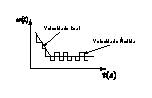
\includegraphics[width=0.5\textwidth]{figuras/ilustracoes/ilustracao_erro_de_quantizacao.eps}
    \caption{Ilustração do erro de quantização na medição de velocidade de rotação.}
    \label{fig:ilustracao_erro_quantizacao}
    \fonte{Própria.}
\end{figure}

A Figura \ref{fig:ilustracao_erro_quantizacao} ilustra um exemplo de medição de velocidade com erro de quantização.\\

Nota-se pela Equação \ref{eq:erro_de_quantizacao_frequencimetro} que o erro de quantização para a medição por frequência decresce com o aumento do número de pulsos por revolução e/ou com o aumento da janela de tempo ($T$), porém o aumento do período de observação acrescenta um atraso na medição da velocidade. O erro relativo à velocidade pode ser descrito como a seguir:

\begin{equation}
    e_{\omega} = \frac{2\pi}{\omega N_{PR} T}
    \label{eq:erro_relativo_quantizacao_frequencimetro}
\end{equation}

Pela Equação \ref{eq:erro_relativo_quantizacao_frequencimetro} observa-se que o erro relativo decresce conforme a velocidade $\omega$ aumenta, ou seja, o erro de quantização será mais significante para baixas velocidades.\\

O outro método de leitura dos \emph{encoders} incrementais é por medição de intervalos de tempo de um mesmo pulso (\textbf{periodímetro}) (ver Figura \ref{fig:ilustracao_periodimetro}). A seguinte formulação pode ser obtida considerando a velocidade do motor constante e sem levar em conta o sentido de giro:

\begin{equation}
    \omega = \frac{d\theta}{dt} \cong \frac{\Delta{\theta}}{nT_{hf}} \cong \frac{2\pi}{N_{PR} n T_{hf}} [rad.s^{-1}] \xrightarrow{} \frac{60}{N_{PR} n T_{hf}} [RPM]
    \label{eq:omega_periodimetro}
\end{equation}

O período entre pulsos será:

\begin{equation}
    T_{\omega}(\omega) = \frac{2\pi}{N_{p}\omega} [s]
\end{equation}

Uma aproximação para o pior caso do erro de quantização relativo a velocidade é apresentado a seguir \cite{analise_incr_enc}:

\begin{equation}
    e_{\omega} = \frac{T_{hf}}{ \frac{2\pi}{N_{PR} \omega} - T_{hf} } \cong \frac{\omega N_{PR} T_{hf}}{2\pi}
    \label{eq:erro_quantizacao_periodimetro}
\end{equation}

A Equação \ref{eq:erro_quantizacao_periodimetro} mostra que o erro é diretamente proporcional à velocidade e a quantidade de pulsos por revolução ($N_{PR}$) e decresce com o aumento da frequência do contador de alta frequência (diminuição de $T_{hf}$).


\begin{figure}[H]
    \centering
    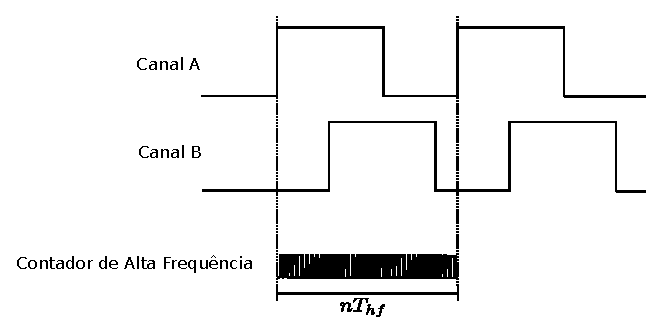
\includegraphics[width=0.5\textwidth]{figuras/ilustracoes/ilustracao_medicao_encoder_por_periodo.eps}
    \caption{Ilustração de leitura de \emph{encoder} periódica.}
    \label{fig:ilustracao_periodimetro}
    \fonte{Própria.}
\end{figure}

Já para se obter o \textbf{sentido da velocidade $\omega$} é necessário fazer uso do padrão binário gerado pelas bordas dos sinais em quadratura. A Figura \ref{fig:cw_signal} ilustrado os sinais em quadratura para uma rotação no sentido horário e destaca o padrão binário gerado nas bordas. A Figura \ref{fig:ccw_signal} ilustra os sinais no sentido anti-horário. O padrão de dois bits é apresentado na Tabela \ref{tab:tabela_simple_code}. \\

\begin{figure}[H]
    \centering
    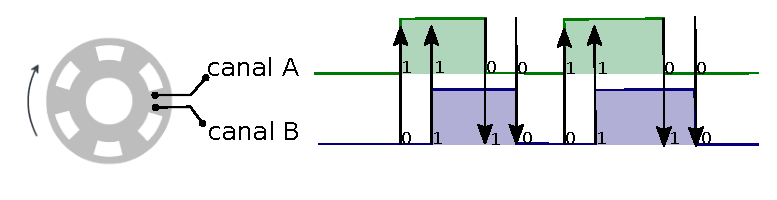
\includegraphics[width=0.7\textwidth]{figuras/ilustracoes/sinal_enquadratura_sentido_CW.eps}
    \caption{Sinal em quadratura para rotação no sentido horário.}
    \label{fig:cw_signal}
    \fonte{Própria.}
\end{figure}

\begin{figure}[H]
    \centering
    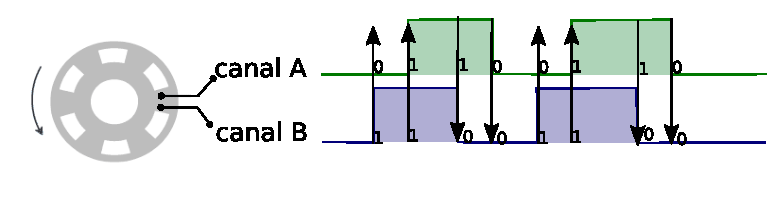
\includegraphics[width=0.7\textwidth]{figuras/ilustracoes/sinal_enquadratura_sentido_CCW.eps}
    \caption{Sinal em quadratura para rotação no sentido anti-horário.}
    \label{fig:ccw_signal}
    \fonte{Própria.}
\end{figure}

% Please add the following required packages to your document preamble:
% \usepackage{graphicx}
\begin{table}[H]
\centering
\resizebox{0.5\textwidth}{!}{%
\begin{tabular}{cc|cc}
\multicolumn{2}{c|}{\textbf{\begin{tabular}[c]{@{}c@{}}Sentido\\     Horário\end{tabular}}} &
  \multicolumn{2}{c}{\textbf{\begin{tabular}[c]{@{}c@{}}Sentido\\ Anti-Horário\end{tabular}}} \\ \hline
\textbf{A} & \textbf{B} & \textbf{A} & \textbf{B} \\
1          & 0          & 1          & 0          \\
0          & 1          & 0          & 1         
\end{tabular}%
}
\caption{Código de 2 bits para identificar o sentido de rotação.}
\label{tab:tabela_simple_code}
\end{table}


\begin{comment}
% Speed Measumment Using Rotary encoders
% for High Performance ac Drives

SPEED MEASUREMENT USING A PERIODIMETER

If we use a periodimeter, we will get the speed not by counting pulses from the encoder, but by counting a high frequency (HF) clock

Let $\alpha_p$ be the corresponding angle to the higher part of an encoder pulse (half of its period), t the period of the HF clock, and n the number of HF pulses arrived at the HF counter. Then, the time spent on an encoder pulse, $T_e$ is:

\begin{equation}
    T_e = n t
\end{equation}

Rotor speed can be obtained as:

\begin{equation}
    \omega_{rotor} = \frac{\alpha_p}{T_e}
\end{equation}

As with the frequencimeter, here also there is a quantization error because of the time T,, which will be always an integer multiple of t With a fixed HFclock frequency, this error will increase as n decreases, that is, as the encoder rotates faster, but it provides accurate measurements at lower speeds. Because the variable with quantization noise is now in the denominator, its effects are much more important than in the frequencimeter.

An additional advantage at low speed is that, as it only needs one pulse to get the speed, the delay is minimal, which is very important at lower speeds.

It also possible to use quadruple frequency. Of course, this reduces the precision, and therefore the maximum velocity where this method is suitable, but also, and this is much more important, it reduces the delay obtaining the velocity when the motor works at low speed. Nevertheless, this method produces stability problems in the zero speed cross. Figure 8 shows an inversion with two possible situations in the encoder output signals. Supposing that there is no quadruple frecuency, and PHASE A controls the HF counter, we see that at the encoder pulse end, the counter has a wrong value, because about half of the HF pulses arrived on each direction of rotation.

The accuracy of the periodimeter is, more than the frequencimeter, related to the accuracy of the encoder, which in general depends on the errors in the radial grating, and the eccentricity of the graduated disk to the bearing.

% Speed Measurement Algorithms for
% Low-Resolution Incremental encoder Equipped
% Drives: a Comparative Analysis


At very low speed the number of high frequency pulses can be extremely high and saturation of the digital timer employed for measurement can occur. Also a speed sample is not available each speed control period, needing an adaptation of the control parameters. In that situation, the quadrature decoding of the encoder pulses can be exploited in order to reduce the width of the measuring window by a factor of four or a reduction of the frequency of the timer can be considered.

The former solution allows to reduce the speed sampling period and improve the control performance of the drive, but makes the measuring system more sensitive to sensor nonidealities, including variations in the transition locations from their nominal values and phasing errors between encoder channels. When low-cost and low-resolution sensors are employed, nonidealities play the major role in the determination of period measuring errors and has to be carefully analysed in drive design phase. The latter solution needs to switch on-line the frequency of the timer and adapt the coeffients of the equations above.

The implementation of the period measuring method is also straightforward as it requires a simple timer capture unit, commonly found inside recent microcontrollers.

% A Simple Speed Feedback System for Low Speed
% DC Motor Control in Robotic Applications

The relationship between the measured frequency using PIC microcontroller and the percentage error is shown in Fig. 2. The percentage error is given as:

\begin{equation}
    e\% = \frac{F_m - F_a}{F_a}.100
\end{equation}

where F m and F a denote the measured and actual frequencies. It is observed that as the frequency increases, the error in the frequency measured from PIC increases linearly, that is, there is a linear relationship between error and frequency.

\end{comment}
\section{Bluetooth}
\label{sec:bluetooth}
% Breve introdução à historia do bluetooth e utilidade
% destacar: custo energético, velocidade de operação, robustez a interferências
A  tecnologia \emph{Bluetooth}  suporta várias opções de topologia, incluindo conexões simples ponto a ponto. Operando na faixa de frequência industrial, científica e médica de $2,4$ GHz, a tecnologia \emph{Bluetooth} suporta várias opções de rádio.

O rádio \emph{Bluetooth} BR/EDR opera com baixo consumo de energia e também utiliza uma abordagem robusta de \textit{Adaptive Frequency Hopping}, transmitindo dados por $79$ canais. O \textit{Bluetooth} BR/EDR inclui várias opções de configuração para a camada física (\emph{PHY}) que suportam taxas de dados de $1$ Mb/s a $3$ Mb/s e suporta vários potências de transmissão, de $1$ mW a $100$ mW, além de várias opções de segurança.
% aprofundar mais? 
\section{Modulação por Largura de Pulso}
\label{sec:PWM}
% Resumo sobre PWM

\emph{Pulse Width Modulation} (PWM) refere-se a um sinal digital pulsante. Esse sinal é utilizado, por exemplo, para simular uma saída analógica em microcontroladores e por isso geralmente é muito usado para o controle de atuadores elétricos como motores, aquecedores, dentre outras coisas, como o controle do brilho de LEDs. \\

A modulação \emph{PWM} pode ser vista como uma maneira de codificar digitalmente níveis de sinal analógico. Nesta técnica, através do uso de contadores de alta resolução, o ciclo de trabalho de uma onda quadrada é modulado para codificar um nível de sinal analógico específico para que então ele atenda os requisitos de uma aplicação desejada. O tempo de ativação é o tempo durante o qual a alimentação CC é aplicada (sinal em nível alto) à carga e o tempo de desativação é o período durante o qual a alimentação é desligada (sinal em nível baixo). Dada uma largura de banda suficiente, qualquer valor analógico pode ser codificado com \emph{PWM}.